\begin{subsection}{Operaciones de la Arquitectura}
    En este punto ya se ha formado el SDDC, la configuración de la infraestructura física y de todos sus componentes está lista para desplegar los componentes que habiliten el servicio Cloud de aprovisionamiento de recursos. Este último paso se completará con los productos agrupados bajo VMware vRealize Suite. Se utilizarán tres des estos productos, vRealize Operations Manager(vROps), Workspace One Access (WSA) y vRealize Automation (vRA).
    % En este punto ya se ha formado el SDDC, la configuración de la infraestructura física y de todos sus componentes está lista para desplegar los componentes que habiliten el servicio Cloud de aprovisionamiento de recursos. Este último paso se completará con los productos agrupados bajo VMware vRealize Suite. Se utilizarán tres des estos productos, vRealize Suite Lifecycle Manager (vRSLCM), Workspace One Access (WSA) y vRealize Automation (vRA).
    %  y, para aprovechar las ventajas de VMware NSX-T y las redes virtuales existentes, utilizarán como red de acceso el Segment \textit{mgmt-xRegion01-VXLAN}.
    % estos proporcionarán un servicio de autenticación centralizado para los usuarios y servicio de aprovisionamiento de recursos
    % El entorno ya está configurado para funcionar como un SDDC, a partir de este punto ya no es necesario realizar ninguna modificación en la infraestructura física ya que todas las tareas que se deben realizar están dentro del alcance de los componentes de VMware Cloud Foundation. Para finalizar la construcción del SDDC y habilitar un servicio donde los usuarios puedan aprovisionar recursos bajo demanda, se instalarán sobre el entorno desplegado las aplicaciones Workspace ONE Access \footnote{VMware vRealize Identity Manager} (WSA) y VMware vRealize Automation (vRA). La primera permite al administrador conectar con el servidor de usuarios Active Directory y gestionarlos para proveer un servicio de autenticación centralizado a múltiples aplicaciones como VMware vRealize Automation. La segunda aplicación permite a los usuarios aprovisionar recursos de forma automatizada desde un catálogo de recursos. VMware vRealize Suite Licfecycle Manager (vRSLCM) es el componente que permite administrar vRA y WSA, su instalación y actualizaciones, las contraseñas de administrador y sus certificados, para ello necesita comunicarse con VMware vCenter Server. Se desplegará una instancia de cada componente en el \textit{management domain} creado anteriormente y estarán conectadas al \textit{segment}/subred \textit{Mgmt-xRegion01-VXLAN}.
    % \begin{subsubsection}{vRealize Operations Manager}
    %     vROps se instala en el entorno para establecer un sistema de valoración de los recursos. Gracias a este componente, el administrador del SDDC será capaz de establecer una valoración de los recursos consumidos por los usuarios con el fin de establecer un límite de consumo total para cada usuario. Además, también permitirá al administrador del SDDC acceder a estadísticas y eventos donde vROps analiza información obtenida de la infraestructura para detectar problemas, proponer soluciones y monitorizar el uso de recursos. vROps monitoriza y obtiene métricas de los recursos disponibles en VMware vCenter Server, VMware NSX-T y VMware vSAN para recopilar los eventos e información de cada uno de ellos con el objetivo de predecir posibles problemas y automatizar la aplicación de soluciones. Además, se integra con vRealize Automation para mostrar al usuario en su portal de acceso información sobre los recursos que utiliza.
    %     \\
    %     \begin{figure}[h]
    %         \centering
    %         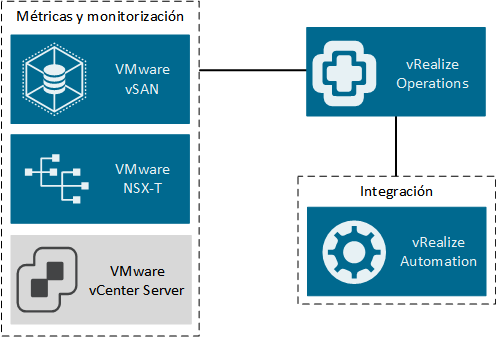
\includegraphics[width=0.4\textwidth]{imaxes/pruebaconcepto/vrealize/estructura-vrops.png}
    %         \caption{Componentes con los que se comunica vROps.}
    %         \label{fig:vrops-components}
    %     \end{figure}
    %     \FloatBarrier
    %     El sistema de valoración que se puede habilitar con vROps consiste en que se establecen una serie precios en una divisa determinada. Por el uso de CPU, memoria RAM y almacenamiento se establece un precio y a medida que los usuarios utilicen el servicio Cloud, vROps se encargará de calcular el precio total de los recursos que ha consumido cada usuario durante un periodo e tiempo. De esta forma el administrador puede obtener una métrica de cuantos ha consumido un usuario y, en caso de que supere un límite establecido poder actuar en consecuencia reduciendo la cantidad de recursos disponibles para el usuario o no permitirle su uso temporalmente.
        % vRSLCM es el primer componente que se instala ya que es el encargado de gestionar el ciclo de vida de los productos de VMware vRealize Suite, incluyendo su despliegue, actualizaciones y gestión de las credenciales de administración, certificados y licencias, por lo tanto permite al administrador del SDDC controlar de forma centralizada la configuración y seguridad de los servicios dedicados a las operaciones del SDDC. Para llevar a cabo sus funciones, vRSLCM debe comunicarse con la instancia de VMware vCenter Server desplegada en el Management Domain.
        % vRSLCM es el primer componente que se instala ya que es el encargado de gestionar el ciclo de vida de los productos de VMware vRealize Suite, incluyendo su despliegue, actualizaciones y gestión de las credenciales de administración, certificados y licencias, por lo tanto permite al administrador del SDDC controlar de forma centralizada la configuración y seguridad de los servicios dedicados a las operaciones del SDDC. Para llevar a cabo sus funciones, vRSLCM debe comunicarse con la instancia de VMware vCenter Server desplegada en el Management Domain.
        % este componente está dedicado a mantener su seguridad y configuración, y a controlar que servicios se encuentran en el entorno, todo para simplificar y facilitar las tareas del administrador. Para llevar a cabo sus funciones, vRSLCM debe mantener una comunicación con la instancia de VMware vCenter Server desplegada en el Management Domain.
        % \begin{figure}[h]
        %     \centering
        %     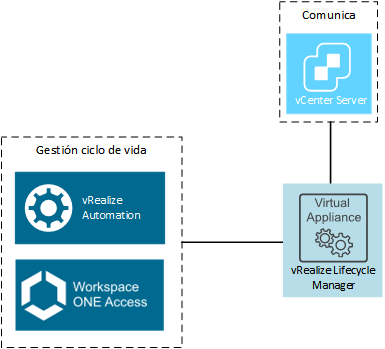
\includegraphics[width=0.4\textwidth]{imaxes/pruebaconcepto/vrealize/diseno-vrlscm.png}
        %     \caption{Componentes con los que se comunica vRSLCM.}
        %     \label{fig:vrealize-components}
        % \end{figure}
        % \FloatBarrier        
        % Durante el despliegue de WSA y vRA, desde vRSLCM se establece su configuración, indicando la licencia, credenciales del administrador, direcciones IP, configuración DNS y NTP, y certificados\footnote{El certificado de cada aplicación es generado manualmente desde la CA y luego subido a vRSLCM, que en este caso es la VM con Windows Server 2016.} para habilitar el acceso seguro desde el navegador web. Las instancias de cada componente desplegado se colocan dentro del cluster vSphere\footnote{\nameref{subsubsec:diseno-vsphere}} creado anteriormente, y utilizarán uno de los Segments creados en VMware NSX-T para conectarse a la red\footnote{Figura \ref{fig:two-tier-topology}}.
% Además, se debe elegir la ubicación donde se van a desplegar las VMs de estos servicios, es decir, el dominio de VMware vCenter Server, el cluster vSphere, la red y el datastore para el almacenamiento.
        
        % En el entorno de pruebas, de cada servicio se crea una instancia en el Management Domain. Cada una se coloca en el cluster vSphere (\nameref{subsubsec:diseno-vsphere}), utilizan el datastore de VMware vSAN (\nameref{subsubsec:diseno-vsan}) y están controladas por la instancia de VMware vCenter Server (\nameref{subsubsec:diseno-vcenter}). Como ya se ha mencionado, las instancias se conectan a un Segment controlado por VMware NSX-T (como se muestra en la figura \ref{fig:two-tier-topology}) para poder hacer uso de sus servicios de red.
        % \begin{figure}[h]
        %     \centering
        %     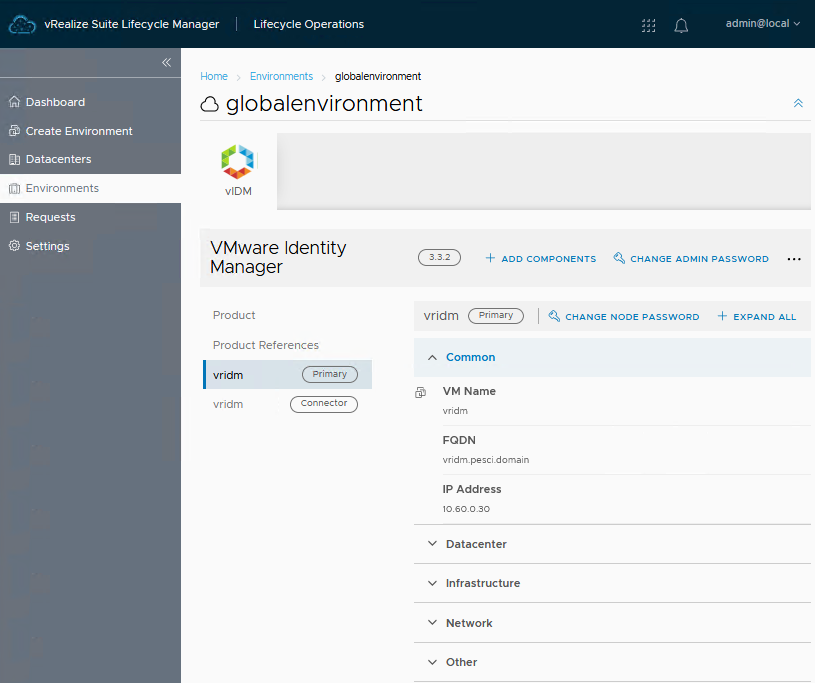
\includegraphics[width=0.6\textwidth]{imaxes/pruebaconcepto/vrealize/config-istance-vridm.png}
        %     \caption{Apartado donde se muestra la configuración de la instancia de WSA en vRSLCM.}
        %     \label{fig:config-WSA}
        % \end{figure}
        % \FloatBarrier
        
        % Dentro de vRSLCM, los despliegues son organizados por entornos pudiendo crearse un entorno por cada servicio o un entorno con todos los servicios. Existen dos modos de despliegue, uno donde se crean tres instancias del servicio para balancear la carga\footnote{El balanceo de la carga se realiza con el servicio de Load Balancing de VMware NSX-T.}, y otro donde solo se crea una instancia.

        % En el entorno, se despliega una instancia de cada servicio. Estas están colocadas bajo el dominio de la instancia de VMware vCenter en el cluster vSphere

        % Este se instala desde SDDC Manager, pero una vez instalado es utilizado para desplegar cualquier servicio de VMware vRealize Suite.
    % \end{subsubsection}
    \begin{subsubsection}{Workspace One Access}
        \label{subsubsec:WSA}
        WSA permite integrar un directorio de usuarios para proporcionarles acceso al servicio Cloud. Así, en el entorno real del CITIC, WSA estaría integrado con el directorio de usuarios de la UDC para que estos pudieran acceder al servicio de aprovisionamiento utilizando las credenciales de la UDC.\\
        En el entorno de pruebas, WSA está integrado con el directorio de usuarios Active Directory situado en la VM con Windows Server 2016. Este Active Directory contiene perfiles de usuarios y grupos de usuarios organizados en unidades organizativas. Los perfiles de usuario se añaden a grupos de usuarios y la creación y mantenimiento de sus credenciales se realiza desde el propio Active Directory. Desde WSA se seleccionan los usuarios y grupos de usuarios que se quieren sincronizar, para habilitarlos dentro del SDDC y posteriormente configurar su acceso a la plataforma de vRA. Como norma general, los permisos y roles se deben aplicar sobre grupos de usuarios y no a perfiles individuales, de esta forma se reduce el tiempo de gestión y se simplifica la estructura del directorio ya que se configura el acceso de un conjunto de usuarios al mismo tiempo.\\
        Los usuarios configurados en el Active Directory son sincronizados en WSA y serán utilizados para mostrar las funcionalidades del servicio Cloud como si se tratase del entorno en producción. Para realizar la sincronización se seleccionarán las unidades organizativas necesarias.
        % , ya que para asignar nuevos permisos a un usuario solo sería necesario añadirlo al grupo correspondiente.        
        % En el Active Directory se han configurado varios usuarios que se sincronizan en WSA. Estos se utilizarán para mostrar las funcionalidades de vRA como si se tratase del entorno real con perfiles de usuarios de la UDC.
        
        \begin{figure}[h]
            \centering
            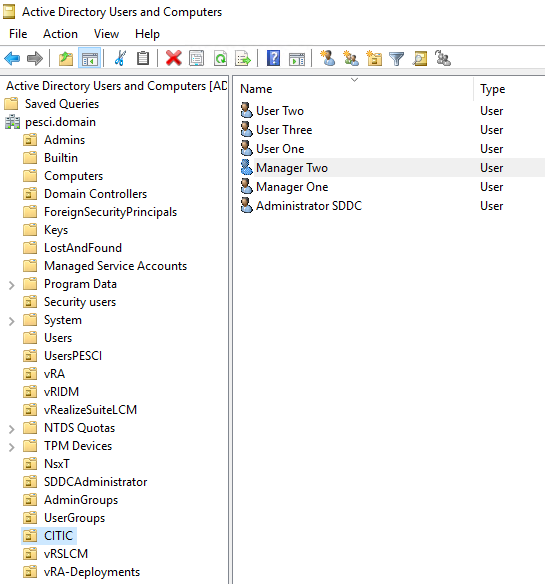
\includegraphics[width=0.6\textwidth]{imaxes/pruebaconcepto/vrealize/UnidadesOrg-Users-AD.png}
            \caption{Unidades organizativas configuradas en el AD junto a los usuarios pertenecientes a la unidad CITIC.}
            \label{fig:users-defined-AD}
        \end{figure}
        \FloatBarrier
        % En WSA se seleccionan aquellas unidades organizativas que se quieren sincronizar. Cada unidad contiene usuarios y grupos de usuarios, los usuarios que harán uso del servicio de aprovisionamiento están colocados en la unidad CITIC.
        \begin{figure}[h]
            \centering
            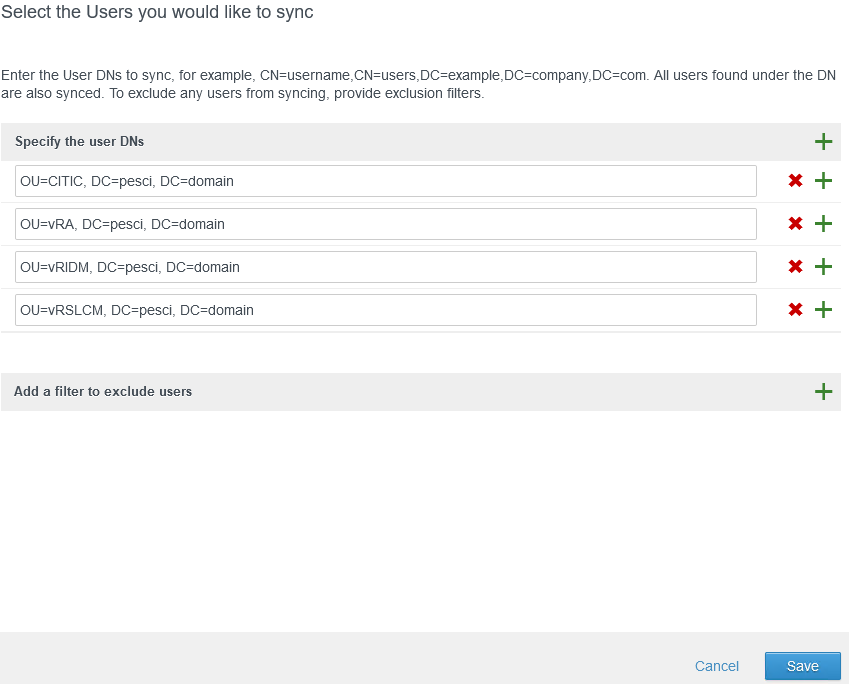
\includegraphics[width=0.6\textwidth]{imaxes/pruebaconcepto/vrealize/syncing-users.png}
            \caption{Sincronización de usuarios desde Workspace One Access seleccionando Unidades Organizativas.}
            \label{fig:users-defined-WSA}
        \end{figure}
        \FloatBarrier
        \begin{figure}[h]
            \centering
            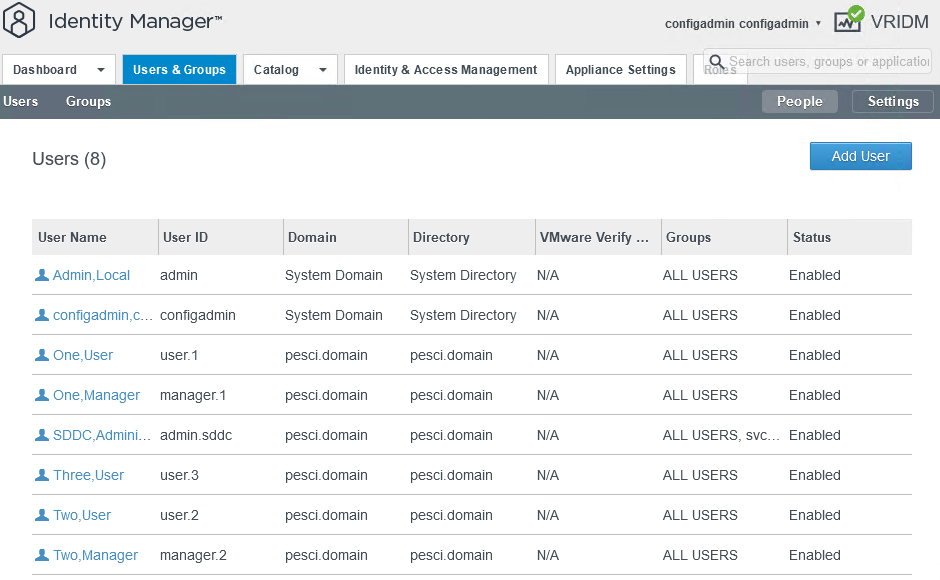
\includegraphics[width=0.6\textwidth]{imaxes/pruebaconcepto/vrealize/users-wsa.png}
            \caption{Usuarios sincronizados en Workspace One Access.}
            \label{fig:users-defined-WSA}
        \end{figure}
        \FloatBarrier
        El acceso al servicio Cloud está centralizado a través de una plataforma de autenticación proporcionada por WSA. Cuando el usuario intenta acceder al servicio este es redirigido a una página web donde introduce sus credenciales, WSA comprueba los datos introducidos y vuelve a redirigir al usuario a la pantalla del servicio. Utilizando esta plataforma  de autenticación el administrador del SDDC puede obtener estadísticas sobre qué usuarios se autentican, a qué servicios acceden y desde dónde lo hacen. Además, también se pueden  modificar los parámetros de autenticación y la configuración las sesiones de usuarios, permitiendo definir si el usuario debe utilizar su cuenta de correo electrónico o nombre de usuario para iniciar sesión o si se utilizan cookies de sesión o persistentes. Por si esto fuera poco, también existe la posibilidad de crear políticas para controlar desde dónde pueden los usuarios acceder al servicio y el tiempo de duración de las sesiones. En la siguiente figura se muestran las reglas de la política por defecto que se aplica, en esta se permite el acceso desde cualquier dirección IP, a través de un navegador web, usando su contraseña y con un tiempo de sesión de 8 horas.
        \begin{figure}[h]
            \centering
            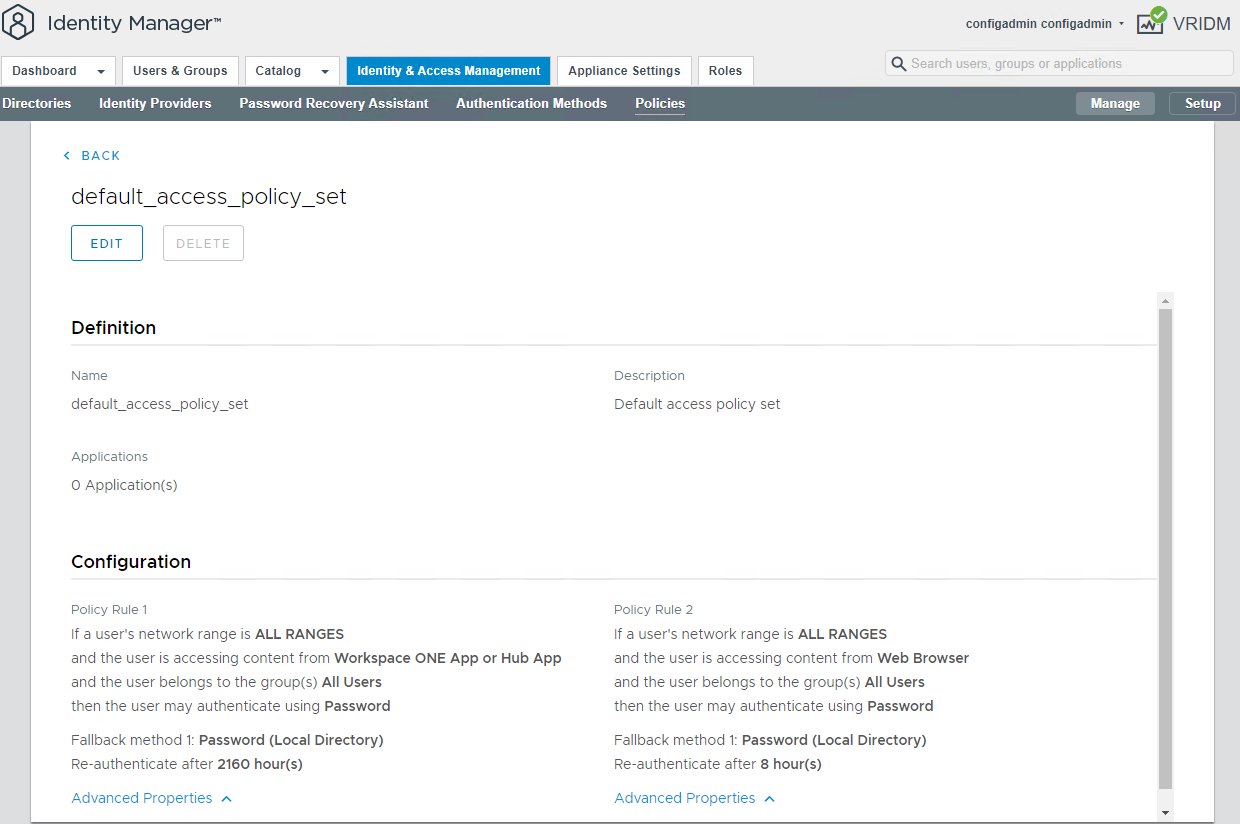
\includegraphics[width=0.6\textwidth]{imaxes/pruebaconcepto/vrealize/default-policy.png}
            \caption{Política de autenticación por defecto establecida en WSA.}
            \label{fig:default-policy}
        \end{figure}
        \FloatBarrier
        \begin{figure}[h]
            \centering
            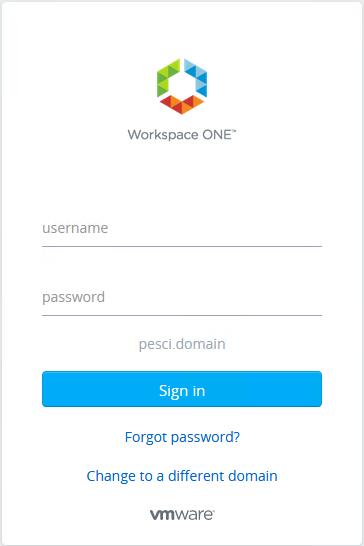
\includegraphics[width=0.3\textwidth]{imaxes/pruebaconcepto/vrealize/wsa-login.png}
            \caption{Plataforma de autenticación de Workspace One Access.}
            \label{fig:wsa-platform}
        \end{figure}
        \FloatBarrier        
        Con WSA el administrador tiene un mayor control sobre los usuarios y cómo estos acceden al servicio Cloud, ya que desde un único punto se gestionan todos los perfiles de usuarios disponibles y la seguridad de acceso, pudiendo controlar qué usuarios acceden y establecer medidas seguridad de forma sencilla. La gestión de las credenciales de cada usuario se separa de la gestión del acceso, ya que lo primero está controlado por el AD y lo segundo por WSA. De esta forma la seguridad del entorno aumenta y las tareas del administrador se simplifican. Con esta plataforma se soluciona uno de los problemas de la infraestructura del CITIC, ya no es necesario crear un perfil manualmente para cada usuario que quiera acceder al servicio y su gestión se centraliza en un componente dedicado a ello.

        % Los usuarios que necesiten acceder a vRA deben estar registrados en el directorio de Workspace One Access. Este componente centraliza el acceso de todos los productos de VMware vRealize. Cuando se despliega se debe configurar un Active Directory que en el caso del entorno está situado en la VM con Windows Server 2016. Dentro del Active Directory existen grupos de seguridad y perfiles de usuario, un perfil de usuario contiene información como nombre, apellidos, dirección e-mail, nombre de usuario y contraseña\footnote{Se pueden configurar más campos pero los que se describen son los obligatorios a la hora de crear un usuario.}, y este puede formar parte de varios grupos de seguridad. Una vez configurado, cada aplicación se conectará a WSA y se podrán asignar roles para los grupos de seguridad y usuarios estableciendo así un nivel de acceso. Además, cada usuario registrado tendrá disponible un catálogo de aplicaciones en el portal de WSA cuyo administrador establecerá que aplicaciones están habilitadas para cada usuario o grupo, eso sí, para que el usuario pueda acceder a ella previamente se debe establecer un rol para ese usuario dentro de la aplicación.

        %*****USUARIOS QUE HAY EN EL ENTORNO Y EL ACCESO A CADA APLICACIÓN*******%
        % \begin{figure}[h]
        %     \centering
        %     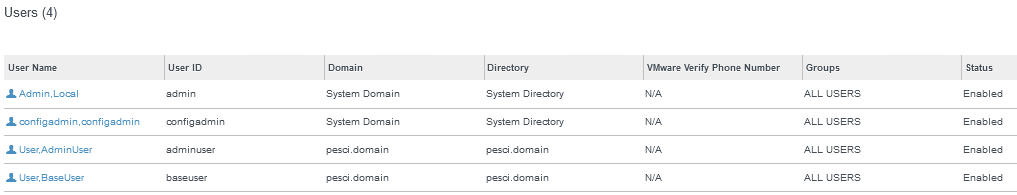
\includegraphics[width=0.4\textwidth]{imaxes/vRealize_pruebaconcepto/usuariosDefinidos.png}
        %     \caption{Muestra los usuarios definidos en el Active Directory sincronizados en Workspace One Access.}
        %     \label{fig:users-defined-AD}
        % \end{figure}
        % \FloatBarrier
        % En la Figura \ref{fig:users-defined-AD} se muestran los dos usuarios definidos en el Active Directory y dos usuarios que se corresponden a los perfiles de administración de WSA, no se utilizarán grupos de seguridad para reducir la complejidad pero su configuración en las aplicaciones de VMware es igual que para los perfiles de usuario. En un entorno real existen usuarios que controlan a otros usuarios y establecen su nivel de acceso, a parte de los perfiles de administrador de cada aplicación. Para el entorno se define el perfil \textit{adminuser} que será el encargado de gestionar el acceso de dos usuarios (\textit{baseuser1} y \textit{baseuser2}) que serán los que consuman a las aplicaciones desplegadas (vRSLCM y vRA). El primero tendrá acceso y permisos de edición en las aplicaciones vRSLCM y vRA, mientras que los dos usuarios base solo podrán acceder a vRA y dentro de este el usuario admin definirá que servicios están habilitados para cada uno.

        %************************************************************************%

    \end{subsubsection}

    \begin{subsubsection}{VMware vRealize Automation}
        VMware vRealize Automation es el componente de VMware vRealize Suite que automatiza el aprovisionamiento de recursos del SDDC. Con esta plataforma los usuarios elaboran diseños de los recursos que necesitan para posteriormente implementarlos y llevar a cabo sus trabajos. Estos diseños,son archivos con formato .yaml en los que se especifican los recursos de la infraestructura que se quieren utilizar y su configuración, como el tamaño de una VM, su sistema operativo, creación de usuarios, instalación de paquetes, redes a las que se conecta, almacenamiento que utiliza o su localización en la infraestructura. Una vez completado el diseño, el usuario lo ejecuta y vRA se encarga de aprovisionar todos los recursos especificados, de forma ordenada, automatizada y transparente. El administrador del SDDC se encargado de establecer qué recursos de la infraestructura están disponibles para los usuarios, asignando a cada uno un tag con la forma \textit{key:value} para que puedan ser referenciados.
        \\        
        Para separar el flujo de trabajo de diferentes usuarios, vRA permite la creación de proyectos que agrupan a un conjunto de usuarios, en los cuales se habilitan diseños a los que solo los miembros del proyecto tienen acceso. En cada proyecto existe el rol de administrador de proyecto y el de miembro de proyecto, el primero es el que se encarga de determinar qué usuarios tienen acceso al proyecto y de habilitar los diseños en un catálogo, el segundo solo tiene acceso a los proyectos donde ha sido admitido para aprovisionar y utilizar los recursos establecidos en los diseños disponibles. El administrador del SDDC se encarga de la creación de cada proyecto y de establecer recursos la cantidad de recursos disponibles para cada uno.
        % Durante proceso de implementación de esos diseños se aprovisionan recursos de forma automática y transparente para el usuario, que puede modificar los requisitos de sus recursos según sea necesario
        % Al mismo tiempo, el administrador establece los límites del diseño/implementación y debe proveer en la infraestructura los medios que se usarán como base para los diseños.
        % En vRA el aprovisionamiento de recursos se realiza a partir de diseños realizados por el usuario. Estos diseños, llamados Blueprints, son archivos con formato .yaml en los que se especifican los recursos que el usuario quiere obtener, estos recursos son VMs, redes y almacenamiento, y para cada recurso definido el usuario puede especificar sus características como el tamaño de una VM y su configuración interna (sistema operativo, instalación de librerías o servicios, redes a las que se conecta). Las blueprints se definen dentro de proyectos en los cuales existen jefes de proyecto y usuarios que utilizan o aprovisionan los recursos definidos en cada blueprint, de esta forma, tanto el administrador como el jefe de proyecto controlan qué usuarios acceden a los recursos de un proyecto. Además, el administrador será el encargado de limitar la cantidad de recursos disponibles para cada proyecto, y de establecer los recursos disponibles para el proyecto, es decir, qué sistemas operativos están disponibles, en qué redes se podrán realizar los despliegues y que datastore utilizarán para el almacenamiento.
        \begin{figure}[h]
            \centering
            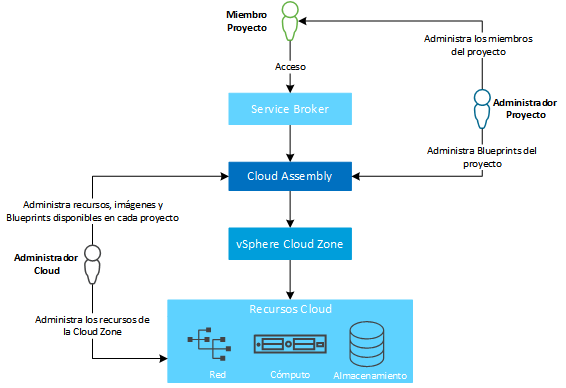
\includegraphics[width=0.7\textwidth]{imaxes/vRealize_pruebaconcepto/ComponentesVRA.png}
            \caption{Uso y componentes de VMware vRealize Automation.}
            \label{fig:vra-components}
        \end{figure}
        \FloatBarrier
        Como se muestra en la figura anterior, en vRA existen tres componentes principales que son Service Broker, a través del cual los usuarios tienen acceso a los diseños e implementaciones de sus proyectos, Cloud Assembly, donde el administrador del SDDC establece los recursos disponibles y donde los administradores de cada proyecto se elaboran de forma automatizada los diseños, y Cloud Zone, punto desde donde vRA accede a la infraestructura para obtener los recursos.
        \\
        vRA soluciona las principales carencias de la infraestructura del CITIC y su servicio de virtualización, que son la falta de automatización en el aprovisionamiento y la falta de control sobre el uso y el acceso a los recursos. Con vRA se proporciona un servicio Cloud de tipo IaaS para la obtención de recursos de forma medida y bajo demanda, mientras el administrador del SDDC puede controlar a qué recursos accede cada usuario y cuantos recursos pueden utilizar mediante el uso del servicio de valoración proporcionado por vROps.
        % \\
        % En la siguiente sección se detallará como se han configurado los recursos de la infraestructura del entorno de pruebas en vRA y cómo son utilizados por los usuarios, ya que esta será la plataforma que complete el servicio Cloud propuesto para la infraestructura del CITIC.
        % Internamente vRA se divide en tres componentes, Cloud Assembly, Service Broker y Cloud Zone.
        % El punto a través del cual los usuarios pueden aprovisionar sus recursos es vRealize Automation. Este producto provee el servicio cloud. 
        % \begin{figure}[h]
        %     \centering
        %     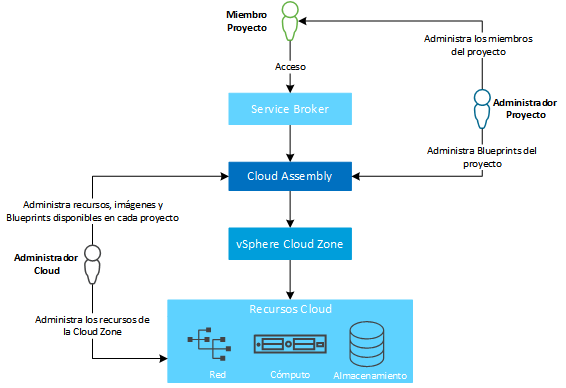
\includegraphics[width=0.8\textwidth]{imaxes/vRealize_pruebaconcepto/ComponentesVRA.png}
        %     \caption{Componentes de VMware vRealize Automation y tareas que realiza cada rol de usuario.}
        %     \label{fig:vra-components}
        % \end{figure}
        % \FloatBarrier
        % Internamente vRA se divide en varios servicios que permiten gestionar los diferentes aspectos de la cloud. Para centrarse en los objetivos de este proyecto solo se hace referencia a dos de esos servicios, el primero es Cloud Assembly el cual permite administrar la infraestructura disponible controlar el uso que se hace de esos recursos, y el segundo es Service Broker, utilizado por los usuarios para aprovisionar los recursos desde un catálogo de plantillas. La obtención de los recursos por parte del usuario se hace desplegando una serie de plantillas llamadas Blueprints diseñadas previamente, en donde se define un conjunto de VMs y recursos de red y de almacenamiento incluyendo otros aspectos como la configuración de cada uno de los recursos, como redes de la infraestructura que se utilizan, cantidad de almacenamiento, o la ubicación del despliegue en la infraestructura. Son ficheros de código con extensión \textit{.yaml} donde se indican etiquetas, aunque también se pueden diseñar con un editor gráfico. Estas plantillas están relacionadas con proyectos, una plantilla pertenece a uno o varios proyectos donde existe un coordinador de proyecto que se encarga de diseñar Blueprints y de administrar los usuarios miembros de ese proyecto. Los proyectos de vRA permiten limitar los recursos para que un conjunto de usuarios pueda desplegar los componentes definidos en las Blueprints disponibles, como la cantidad de memoria RAM, cantidad de instancias que se pueden desplegar y cantidad de almacenamiento, también aquellas redes que se pueden utilizar. Desde el punto de vista de vRA, la infraestructura se divide en Cloud Zones, las cuales son conjuntos de recursos situados en distintos proveedores Cloud que pueden ser públicos como AWS o Azure, o privados que solo pueden ser clusters vSphere. En el caso del entorno desplegado solo se tendrá una única Cloud Zone de tipo vSphere. En cada Cloud Zone se define como se deben distribuir los recursos aprovisionados sobre la infraestructura. 
        % Finalmente será el administrador de la infraestructura el que se encargue de proveer los recursos, administrar los proyectos disponibles, gestionar los coordinadores de cada proyecto y controlar y limitar el uso de los recursos.
        % Finalmente, vRA permite configurar tarjetas donde se puede definir el coste del aprovisionamiento de CPU, almacenamiento y memoria RAM, además del coste de uso de otros elementos como sistemas operativos, el uso de una determinada red o el uso de una determinada Cloud Zone. Estas tarjetas se asignan por proyecto para determinar el coste que tendrá el consumo de recursos por mes.
    \end{subsubsection}
    \begin{subsubsection}{vRealize Operations Manager}
        vROps se instala en el entorno para establecer un sistema de valoración de los recursos. Gracias a este componente, el administrador del SDDC será capaz de establecer una valoración de los recursos consumidos por los usuarios con el fin de establecer un límite de consumo total para cada usuario. Además, también permitirá al administrador del SDDC acceder a estadísticas y eventos donde vROps analiza información obtenida de la infraestructura para detectar problemas, proponer soluciones y monitorizar el uso de recursos. vROps monitoriza y obtiene métricas de los recursos disponibles en VMware vCenter Server, VMware NSX-T y VMware vSAN para recopilar los eventos e información de cada uno de ellos con el objetivo de predecir posibles problemas y automatizar la aplicación de soluciones. Además, se integra con vRealize Automation para mostrar al usuario en su portal de acceso información sobre los recursos que utiliza.
        \\
        \begin{figure}[h]
            \centering
            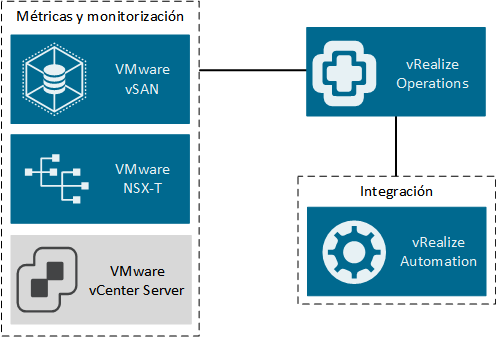
\includegraphics[width=0.4\textwidth]{imaxes/pruebaconcepto/vrealize/estructura-vrops.png}
            \caption{Componentes con los que se comunica vROps.}
            \label{fig:vrops-components}
        \end{figure}
        \FloatBarrier
        El sistema de valoración que se puede habilitar con vROps consiste en que se establecen una serie precios en una divisa determinada. Por el uso de CPU, memoria RAM y almacenamiento se establece un precio y a medida que los usuarios utilicen el servicio Cloud, vROps se encargará de calcular el precio total de los recursos que ha consumido cada usuario durante un periodo e tiempo. De esta forma el administrador puede obtener una métrica de cuantos ha consumido un usuario y, en caso de que supere un límite establecido poder actuar en consecuencia reduciendo la cantidad de recursos disponibles para el usuario o no permitirle su uso temporalmente. Esta información sobre cuantos recursos ha consumido un usuario es accesible por el administrador del SDDC y por el propio usuario desde el portal de vRealize Automation.
        \\
        Con este componente se completa el servicio Cloud al añadir un sistema de control sobre el uso de recursos, hasta ahora inexistente en el servicio del CITIC. El objetivo de este sistema consiste en optimizar al máximo rendimiento de la infraestructura evitando que los usuarios tengan recursos reservados y que en realidad no están siendo usados. De esta forma se pueden liberar esos recursos ociosos y ponerlos a disposición del resto de usuarios.
    \end{subsubsection}

    
\end{subsection}